\subsection{Path counting}
\label{sec:path_counting}

This section is devoted to counting
the number of ways non-backtracking
walks can be concatenated to obtain a circuit as in 
Section~\ref{sec:matrix_decomp}.
We will follow closely the combinatorial analysis used in 
\citet*{brito2016}. 
In that paper, the authors needed a similar count for 
self-avoiding walks. 
We make the necessary adjustments to our current scenario.
% This is similar to the ``cycling times'' arguments of \citet*{bordenave2015a}.

Our goal is to find a reasonable bound for the number of circuits which
contribute to the trace bound, 
Eqn.~\eqref{eq:trace_bound} and shown graphically in Figure~\ref{fig:circuit}.
Define $\mathcal{C}_{\nvertex, \nedge}^\nvright$ as those circuits
which visit exactly 
$\nvertex = |V(\gamma)|$ different vertices, 
$\nvright = |V(\gamma) \cap V_2|$ of them in the right set, and
$\nedge = |E(\gamma)|$ different edges. Note, these are undirected edges in $E(G)$.
This is a set of circuits of length $2 k \ell$ obtained as the
concatenation of $2k$ non-backtracking,
tangle-free walks of length
$\ell$.
We denote such a circuit as
$\gamma= ( \gamma_1,\gamma_2,\cdots, \gamma_{2k} )$,
where each $\gamma_j$ is a length $\ell$ walk.

To bound $C_{\nvertex, \nedge}^\nvright = | \mathcal{C}_{\nvertex, \nedge}^\nvright |$,
we will first choose the set of vertices and order them.
The circuits which contribute are indeed directed non-backtracking walks.
However, by considering undirected walks along a fixed ordering of vertices,
that ordering sets the orientation of the first and thus the rest of the
directed edges in $\gamma$.
Thus, we are counting the directed walks which contribute to 
Eqn.~\eqref{eq:trace_bound}.
We relabel the
vertices as $1,2, \ldots, \nvertex$ as they appear in $\gamma$.
Denote by $\mathcal{T}_{\gamma}$ 
the spanning tree of those edges
leading to new vertices
as induced by the path $\gamma$.
The enumeration of the vertices tells us how we
traverse the circuit
and thus defines $\mathcal{T}_{\gamma}$ uniquely.

We encode each walk $\gamma_j$
by dividing it into sequences of subpaths of three types,
which in our convention 
{\it must always occur} as type 1 $\to$ type 2 $\to$ type 3,
although some may be empty subpaths.
Each type of subpath is encoded with a number, 
and we use the encoding to upper bound the number of such paths that can occur.
Given our current
position on the circuit, i.e.\ the label of the current vertex, and
the subtree of $\mathcal{T}_{\gamma}$ already discovered 
(over the whole circuit $\gamma$
not just the current walk $\gamma_j$), 
we define the types and their encodings:
\begin{enumerate}[{Type} 1:]
\item These are paths with the property that all of their edges
are edges of $\mathcal{T}_{\gamma}$ and have been traversed already in
the circuit. 
These paths can be encoded by their end vertex.
Because this is a path contained in a tree,
there is a unique path connecting its initial and final vertex. 
We use 0 if the path is empty.
\item These are paths with all of their
edges in $\mathcal{T}_{\gamma}$ 
but which are traversed for the first time in the circuit. 
We can encode these paths by their length,
since they are traversing new edges, and we know in what order the
vertices are discovered. 
We use 0 if the path is empty.
\item These paths are simply a single edge, 
not belonging to $\mathcal{T}_\gamma$,
that connects the end of a path of type 1 or 2 
to a vertex that has been already discovered. 
Given our position on the circuit, 
we can encode an edge by its final vertex. 
Again, we use 0 if the path is empty.
\end{enumerate}
Now, we decompose $\gamma_j$ into an ordered sequence of triples
to encode its subpaths:
\[ 
(p_1,q_1,r_1) (p_2,q_2,r_2) \cdots (p_t,q_t,r_t),
\]
where each $p_i$ characterizes subpaths of type 1, $q_i$ characterizes
subpaths of type 2, and $r_i$ characterizes subpaths of type 3.
These subpaths occur in the order given by the triples.
We perform this decomposition using the minimal possible number of triples.

Now, $p_i$ and $r_i$ are both numbers in $\{0,1,...,\nvertex \}$, since
our cycle has $\nvertex$ vertices. On the other hand, $q_i \in \{ 0,1,...,\ell \}$
since it represents the length of a subpath of a non-backtracking
walk of length $\ell$. 
Hence, there are  $(\nvertex + 1)^2 (\ell+1)$ possible triples. 
Next, we want to bound how many of these triples occur in $\gamma_j$. 
We will use the following lemma.

\begin{lemma} 
Let $(p_1,q_1,r_1) (p_2,q_2,r_2) \cdots (p_t,q_t,r_t)$ 
be a minimal encoding of a non backtracking walk $\gamma_j$, as described above. 
Then $r_i = 0$ can only occur in the last triple $i = t$.
\end{lemma}
\begin{proof} 
We can check this case by case. 
Assume that for some
$i<t$ we have $(p_i,q_i,0)$,
and consider the concatenation with
$(p_{i+1},q_{i+1},r_{i+1})$. 
First, notice that both $p_{i+1}$ and
$q_{i+1}$ cannot be zero since then we will have
$(p_i,q_i,0)(0,0,v^*)$ which can be written as $(p_i,q_i,v^*)$. 
If $q_i\neq 0$,
then we must have $p_{i+1} \neq 0$.
Otherwise, we split a path of new edges (type 2),
and the decomposition is not minimal.
This implies that we visit new edges and move to edges
already visited, hence we need to go through a type 3 edge, 
implying that $r_i \neq 0$. 
Finally, if $p_i \neq 0$ and $q_i = 0$, 
then we must have
$p_{i+1}=0$; 
otherwise, we split a path of old edges (type 1). 
We also require
$q_{i+1} \neq 0$, 
but
$(p_i,0,0)(0,q_{i+1},r_{i+1})$ is the same as $(p_i,q_{i+1},r_{i+1})$, 
which contradicts the minimality condition. 
This covers all possibilities and
finishes the proof.
\end{proof}

\begin{figure}
\centering
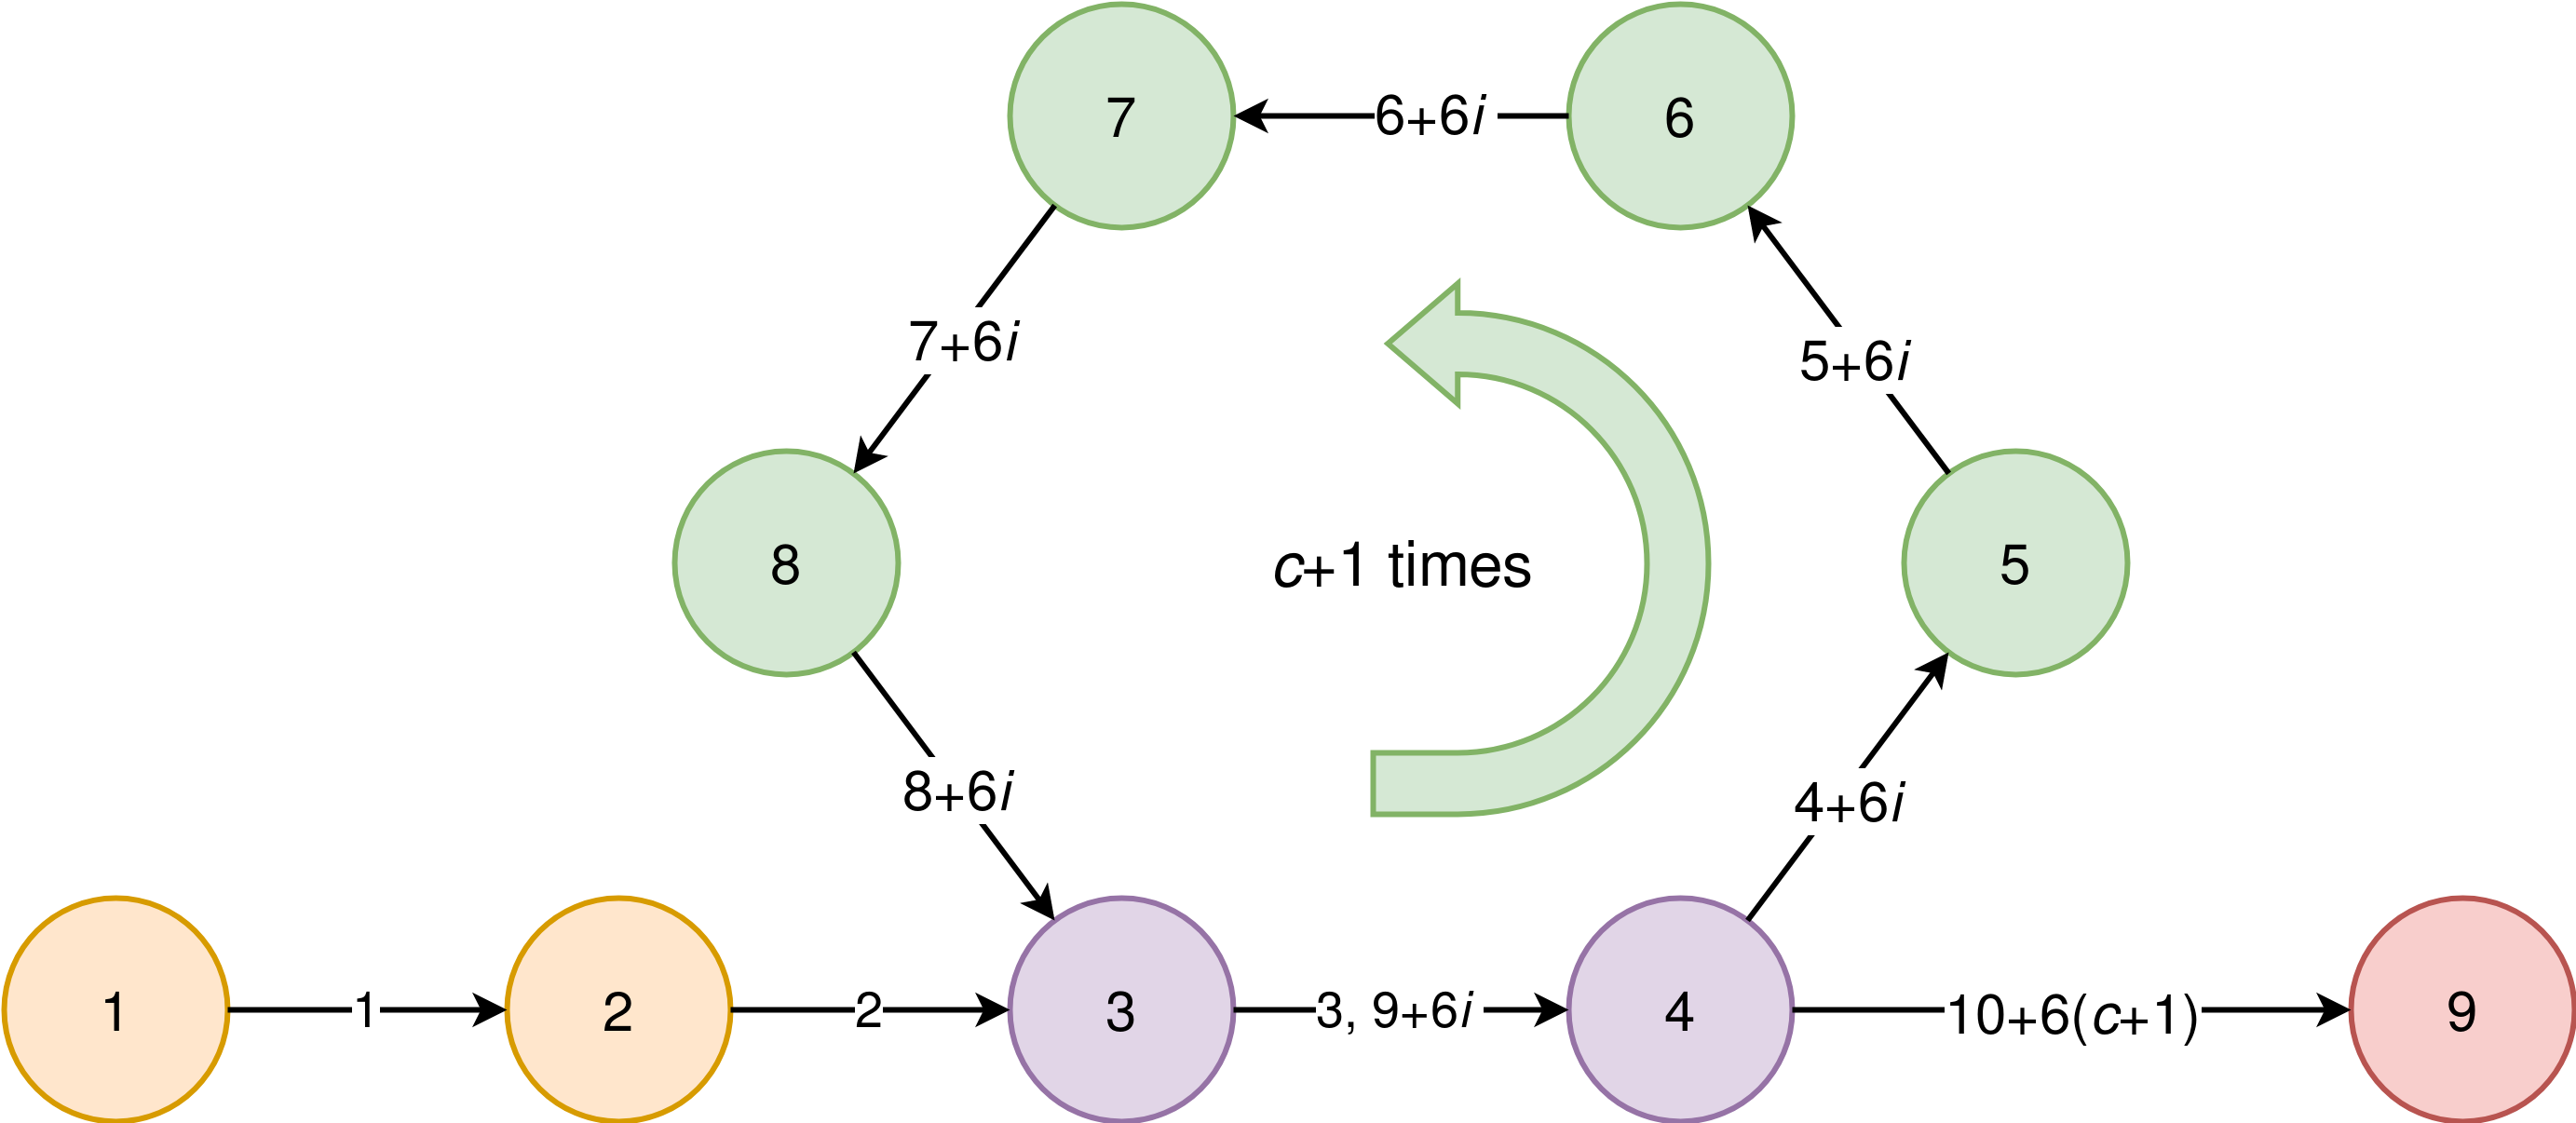
\includegraphics[width=0.75\linewidth]{path_encoding.png}
\caption{
Encoding an $\ell$-tangle-free walk, 
in this case the first walk in the circuit $\gamma_1$, 
when it contains a cycle. 
The vertices and edges are labeled in the order of their traversal.
The segments $\gamma^a$, $\gamma^b$, and $\gamma^c$ occur on edges numbered
$(1, 2, 3)$; $(4 + 6i, 5+6i, 6+6i, 7+6i, 8+6i, 9+6i)$ for $i = 0, 1, \ldots c$;
and $(10+6c)$, respectively.
The encoding is $(0,3,0) | (0,4,3)(4,0,0) \| (0,1,0)$.
Suppose $c = 1$. 
Then $\ell = 22$
and the encoding is of length $3 + (4+1+1)(c+1) + 1$, 
we can back out $c$ to find that the cycle is repeated twice.
The encodings become more complicated later in the circuit as vertices 
see repeat visits. 
}
\label{fig:path_encoding}
\end{figure}

Using the lemma, any encoding of a non-backtracking walk
$\gamma_j$ has
at most one triple with $r_i=0$. 
All other triples indicate the
traversing of a type 3 edge. 
We now give a very rough upper bound for 
how many of such encodings there can be. 
To do so, we will use the tangle-free property and
slightly modify the encoding of the paths with cycles.
Consider the two cases:
\begin{enumerate}[{Case} 1:]
\item {Path $\gamma_j$ contains no cycle.} 
This implies that we traverse each edge within
$\gamma_j$ once. 
Thus, we can have at most $\chi= \nedge - \nvertex + 1$ many
triples with $r_i\neq 0$. 
This gives a total
of at most
\[ 
 \left((\nvertex+1)^2 (\ell+1) \right)^{\chi+1}
\]
many ways to encode one of these paths.
\item 
{Path $\gamma_j$ contains a cycle.} 
Since we are dealing with non-backtracking, tangle-free walks, 
we enter the cycle once, 
loop around some number of times, 
and never come back. 
We change the encoding of such paths slightly. 
Let $\gamma_j^{a}$, $\gamma_j^{b}$, and $\gamma_j^{c}$
be the segments of the path before, during, and after the cycle.
We mark the start of the cycle with $|$ and its end with $\|$. 
The new encoding of the path is:
\[ 
(p^a_1,q^a_1,r^a_1) \cdots (p^a_{t^a},q^a_{t^a},r^a_{t^a}) 
\, | \,
(p^b_1,q^b_1,r^b_1) \cdots (p^b_{t^b},q^b_{t^b},r^b_{t^b}) 
\, \| \,
(p^c_1,q^c_1,r^c_1) \cdots (p^c_{t^c},q^c_{t^c},r^c_{t^c}),
\]
where we encode the segments separately. 
Observe that each a subpath is connected and self-avoiding.
The above encoding tells
us all we need to traverse $\gamma_j$,
including how many times to loop around the cycle:
since the total length is $\ell$, 
we can back out the number of circuits around the cycle
from the lengths of $\gamma_j^{a}$, $\gamma_j^{b}$, and $\gamma_j^{c}$.
See Figure~\ref{fig:path_encoding}.
Following the analysis made for Case 1, 
the subpaths $\gamma_j^{a}$, $\gamma_j^{b}$, $\gamma_j^{c}$
are encoded by at most $\chi + 1$ triples,
but we also have at most $\ell$ choices each for our marks
$|$ and $\|$. 
We are left with at most
\[
 \ell^2 \left((\nvertex+1)^2 (\ell+1) \right)^{\chi+1}
\]
ways to encode any path of this kind.
\end{enumerate}
Together, these two cases mean there are less than
$
%2 \ell^2 \left((\nvertex+1)^2 (\ell+1) \right)^{\chi+1} \leq
2 \ell^2 \left((\nvertex+1)^2 (\ell+1) \right)^{\chi+1}
$
such paths.

Now we conclude by encoding the entire circuit 
$\gamma = (\gamma_1, \ldots, \gamma_{2k})$.
We first choose $\nvertex$ vertices, $\nvright$ in the set $V_2$, and order them,
which can occur in 
$(m)_\nvright (n)_{\nvertex-\nvright} \leq m^\nvright n^{\nvertex - \nvright}$ different ways. 
Finally, in the whole path $\gamma$ 
we are counting concatenations of
$2k$ paths which are $\ell$-tangle-free.
Therefore, we conclude with the following Lemma:

\begin{lemma}
\label{lem:circuit_count}
Let $\mathcal{C}_{\nvertex, \nedge}^\nvright$ 
be the set of circuits
$\gamma = (\gamma_1, \ldots, \gamma_{2k})$
of length $2 k \ell$ obtained as the
concatenation of $2k$ non-backtracking,
tangle-free walks of length
$\ell$,
i.e.\ $\gamma_s \in F^\ell$ for all $s \in [2k]$,
which visit exactly 
$\nvertex = |V(\gamma)|$ different vertices, 
$\nvright = |V(\gamma) \cap V_2|$ of them in the right set, and
$\nedge = |E(\gamma)|$ different edges.
If $C_{\nvertex, \nedge}^\nvright = |\mathcal{C}_{\nvertex, \nedge}^\nvright|$, then
\begin{equation}
C_{\nvertex, \nedge}^\nvright
\leq
m^\nvright n^{\nvertex - \nvright} (2 \ell)^{4k} 
\left( (\nvertex+1)^2 (\ell+1) \right)^{2k (\chi + 1)},
\end{equation}
where $\chi = \nedge - \nvertex + 1$.
\end{lemma}

The circuits that contribute to the remainder term
$R^{\ell, j}$ 
are slightly different.
In this case, each length $\ell$ segment
is an element of $T^{\ell, j}$ rather than $F^{\ell}$.
We have to slightly modify the previous argument for this case.

\begin{lemma}\label{lem:combinatorial_of_reminder}
Let $\mathcal{D}_{\nvertex,\nedge}^\nvright$ 
be the set of circuits
$\gamma = (\gamma_1, \ldots, \gamma_{2k})$
of length $2k\ell$
obtained as the concatenation
of $2k$ elements 
$\gamma_s \in T^{\ell, j}$
for $s = 1, \ldots, 2k$,
that visit exactly $\nvertex$ vertices, 
$\nvright$ of which are in $V_2$, and $\nedge$ different edges. 
Then for $D_{\nvertex,\nedge}^\nvright = | \mathcal{D}_{\nvertex,\nedge}^\nvright |$,
we have
\begin{align}
\label{bound:D}
D_{\nvertex,\nedge}^\nvright
\leq
m^\nvright n^{\nvertex-\nvright}
(2 \ell)^{6k} 
( (\nvertex + 1)^2 (\ell + 1) )^{6k(\chi + 1)} .
\end{align}
\end{lemma}

\begin{proof}
Since each 
$\gamma^s = (e_1, \ldots, e_{2\ell + 1}) \in T^{\ell,j}$,
we have that
$\gamma' = (e_1, \ldots, e_{2j-1}) \in F^{j-1}$,
$\gamma'' = (e_{2j-1}, e_{2j}, e_{2j+1}) \in F^{1}$,
and $\gamma''' = (e_{2j+1}, \ldots, e_{2\ell + 1}) \in F^{\ell - j}$.
Encoding $\gamma'$, $\gamma''$, and $\gamma'''$ as before,
we have the generous upper bound of at most
\[
\left[ (2\ell) ((\nvertex + 1)^2(\ell+1))^{\chi+1} \right]^3
\]  
many encodings for each $\gamma_s$. 
Choosing and ordering the vertices, then concatenating $2k$ of these paths gives
the final result.
\end{proof}


\subsection{Half edge isomorphism counting}
   
We have constructed the circuits in 
$\mathcal{C}_{\nvertex, \nedge}^\nvright$
and
$\mathcal{D}_{\nvertex, \nedge}^\nvright$
by choosing the vertices and edges that participate in them.
However, the expectation bound applies to matchings
of half-edges in the configuration model.
Since there are multiple ways to configure the half edges 
into such a circuit, this must
be taken into account in the combinatorics.

\begin{lemma}
\label{lem:edge_iso}
Let $I_{\nvertex, \nedge}^\nvright$
be the number of half edge choices for the graph
induced by
$\gamma \in \mathcal{C}_{\nvertex, \nedge}^\nvright
\cup \mathcal{D}_{\nvertex, \nedge}^\nvright$.
Then,
\begin{equation}
    I_{\nvertex, \nedge}^\nvright 
    \leq 
    d_1^{\nvertex - \nvright} 
    (d_1 - 1)^{\nedge - \nvertex + \nvright}
    d_2^{\nvright}
    (d_2 - 1)^{\nedge - \nvright} .
    % (d_1 (d_1 - 1))^{\nvertex - \nvright} 
    % (d_2 (d_2 - 1))^{\nvright}
    % d^{2 (\chi + k)},
\end{equation}
\end{lemma}

\begin{proof}
% First, consider the simple case where every vertex has degree at most two,
% i.e.\ the circuit $\gamma$ is a path.
% For a left vertex we will have $d_1 (d_1 - 1)$ choices for 
% the two half edges which are used in its outgoing edges, 
% and there are $\nvertex - \nvright$ many of them,
% which leads to the term $(d_1 (d_1 - 1))^{\nvertex - \nvright}$.
% Similarly, every right vertex has $d_2 (d_2 - 1)$ choices for 
% the two half edges, 
% and there are $\nvright$ many of them,
% which gives the term $(d_2 (d_2 - 1))^{\nvright}$.

% Now consider the case when some vertices have degree greater than two. 
% These occur due to either cycles in the circuit
% or backtracking.
% Recall that $\chi$ corresponds to the number of 
% fundamental cycles in the circuit.
% Every fundamental cycle either adds one to the degree of two vertices
% or adds two to the degree of one vertex.
% Either of these cases has at most $d^2$ choices for the half edges,
% giving a term of $d^{2\chi}$.
% Every backtrack can add one to the degree of at most one vertex,
% and since the circuit can backtrack at most $2k$ times
% this leads to a term of $d^{2k}$.

For every left vertex $v$, with degree $g_v$ on the graph induced by $\gamma$, 
the number of choices of half edges is $d_1(d_1-1)\dots(d_1- g_v+1)\leq d_1 (d_1-1)^{g_v-1}$. 
Note that the choice of half edges are independent for the left vertices. 
We then get that there are 
$d_1^{\nvertex-\nvright} (d_1-1)^{\nedge - \nvertex+\nvright}$ 
many choices, 
where we used that the sum of all the degrees on one component of a bipartite graph 
equals the number of edges: $\nedge = \sum_v g_v$. 
Similarly, for right vertices we get 
$d_2^{\nvright}(d_2-1)^{(\nedge-\nvright)}$.
\end{proof}

\begin{corollary}
\label{cor:edge_iso}
We have that
\begin{equation}
    I_{\nvertex, \nedge}^\nvright \leq 
    (d_1 (d_1 - 1))^{\nvertex - \nvright}
    (d_2 (d_2 - 1))^\nvright
    (d - 1)^{2 (\chi - 1)}.
\end{equation}
\end{corollary}

\subsection{Bounding the imbalance $\psi$}

We focus now on the quantity defined as 
$\psi = \nvright - \nedge / 2 $. 
Informally, $\psi$ captures the {\it imbalance} between the number of vertices 
on each partition of the bipartite graph visited by the circuit $\gamma$. 
We show that this imbalance is not too large.
\begin{lemma}\label{lem:imbalance}
Let $\ell < \frac{1}{32} \log_d(n)$,
then $\psi \leq 16 k^2$ with high probability.
\end{lemma}
\begin{proof}
For any subgraph $H$ define $\psi(H) = \nvright(H)-\nedge(H)/2$. 
We set $\psi=\psi(\gamma)$. 
To bound this quantity, we analyse the subgraph 
$\gamma_{\leq i}$, 
obtained by the concatenation of the first $i$ walks in $\gamma$,
i.e.\ the union of the graphs induced by $\gamma_1, \ldots, \gamma_i$.
Our choice of $\ell$ 
implies that every neighborhood of radius $4\ell$ is tangle-free with high probability. Hence, every non-backtracking walk $\gamma_j$ 
is either a path or a path with exactly one loop.
It is not hard to conclude that 
$\psi(\gamma_j) \leq 2$ for all $j$ and 
$\psi(\gamma_{\leq 1}) = \psi(\gamma_1) \leq 2$. 
We now proceed inductively to add walks to our graph, one by one, 
as they appear on the circuit.
We will upper bound the increment 
$\psi(\gamma_{\leq i+1}) - \psi(\gamma_{\leq i})$ 
by looking at how the addition of $\gamma_{i+1}$ changes the imbalance. 

To analyse this, consider the intersection of 
$\gamma_{i+1}$ and each $\gamma_j$, $1\leq j\leq i$. 
Notice that $\psi$ may increase only if there are vertices 
at which the two walks split apart. 
We claim that there are at most two such vertices. 
Assume that at $v_1,v_2$ and $v_3$ the two walks split. 
Then there are two disjoint cycles in the union of $\gamma_{i+1}$ and $\gamma_j$, 
obtained by following each first from $v_1$ to $v_2$ 
and then from $v_2$ to $v_3$. 
But this is a contradiction, 
since the diameter of this union is less than $2 \ell < \frac{1}{8} \log(n)$,
which implies that their union is tangle-free. 
We conclude that $\psi(\gamma_{i+1} \cup \gamma_j) \leq 8$
since there are at most two splits and 
each split contributes at most four to the imbalance. 
Then
$\psi(\gamma_{\leq i+1}) \leq \psi(\gamma_{\leq i}) + 8i + 2$,
which implies that $\psi(\gamma)\leq 16k^2$, as desired.
\end{proof}

\subsection{Bounding the inconsistent edges} 
We will need a bound on the number of inconsistent edges of multiplicity one,
which we get in the following lemma. Recall Definition~\ref{def:incon_edges}, which introduced inconsistent edges. 

\begin{lemma} 
Let $b_\mathcal{C}$ 
denote the number of inconsistent edges of multiplicity one 
on a circuit 
$\gamma = (\gamma_1, \ldots, \gamma_{2k})$ 
consisting of $2k$ non-backtracking walks of length $\ell$ each. 
It holds that
$ b_\mathcal{C} \leq 4 (k + \chi)$, 
where $\chi=\nedge-\nvertex+1$.
\label{lem:inconsistent}
\end{lemma}
\begin{proof}
Let $\{e,f\}$ be an inconsistent edge of multiplicity one, where
$e$ and $f$ are its half edges.
For inconsistency and without loss of generality,
there must exist 
another edge
$\{e,f'\}$ in $\gamma$,
so that
$m_\gamma (e) \neq 1$.
We may assume that $\{e,f\}$ is traversed before $\{e,f'\}$. 
Let $v$ be the vertex of $e$ and consider the two possible scenarios:
\begin{enumerate}[{Case} 1:]
    \item There is no cycle containing $v$ in $\gamma$.
    Then the edge $\{e,f\}$ may only be inconsistent
    if $v$ is visited 
    at the end of one of the $2k$ non-backtracking walks $\gamma_i$ and
    $\{e,f'\}$ is at the beginning of $\gamma_{i+1}$. 
    Hence, in this case we have at most two inconsistent edges of multiplicity one. 
    This yields at most $4k$ such edges.
    \item There is a cycle passing through $v$. 
    For each such cycle there is an edge that does not belong to the tree 
    $T_{\gamma}$ (defined in Section~\ref{sec:path_counting}). 
    Furthermore, each cycle creates at most four inconsistent edges. 
    Combining these two facts we get at most $4\chi$ and the proof follows.
\end{enumerate}
\end{proof}

\begin{lemma}\label{lem:inconsistent_edges_reminder}
Consider a circuit $\gamma = (\gamma_1, \ldots, \gamma_{2k})$
with $\gamma_s \in T^{\ell,j}$ for $j \in [2k]$,
with $\gamma_s$ decomposed as $\gamma_s', \gamma_s'', \gamma_s'''$
as in the Definition~\ref{def:tangled_paths}.
Let 
$b_\mathcal{D}$ 
denote the number of inconsistent edges of multiplicity one 
in the union of segments
$\bigcup_{s=1}^{2k} (\gamma_s' \cup \gamma_s'')$.
Then 
$b_\mathcal{D} 
\leq 
16k+4 \chi$, 
where
$\chi = \nedge - \nvertex + 1$.
\label{lem:inconsistent_tangled}
\end{lemma}

\begin{proof}
The argument is similar to the above; however, now there are $4k$ segments
in $\bar\gamma = \bigcup_{s=1}^{2k} (\gamma_s' \cup \gamma_s'')$,
counting $\gamma_s'$ and $\gamma_s''$ separately.
As above, each of these $4k$ segments may yield at most 2 inconsistent edges.
Furthermore, the graph induced by $\bar\gamma$ may not be connected;
let $C$ be the number of connected components.
Each edge that creates a cycle may yield at most 4 inconsistent edges,
and there are at most $\nedge - \nvertex + C$ non-tree edges.
Then, we have that
\[
b_\mathcal{D} 
\leq 8 k + 4 (\nedge - \nvertex + C) 
\leq 8k + 4 (\nedge - \nvertex + 2k)
\leq 16 k + 4 \chi,
\]
as claimed.
\end{proof}

% \textcolor{red}{Is the last equality an inequality? (because of the $-1$ on $\chi$). Also, the proof yields a 16, why do we want a 24? I think the 16 is fine.}
% \todo{For some reason Bordenave, Lemma 21 has 
% the constant 24, 
% do you see why he gets this constant? The constant doesn't end up mattering, however.} \textcolor{red}{He uses $p-1< p\leq 2m$ and gets the 24. In our case we are fine with $16$, like you already pointed out.}